\let\negmedspace\undefined
\let\negthickspace\undefined
\documentclass[journal,12pt,onecolumn]{IEEEtran}
\usepackage{pgfplots}
\pgfplotsset{compat=1.17}
\usepackage{cite}
\usepackage{amsmath,amssymb,amsfonts,amsthm}
\usepackage{algorithmic}
\usepackage{graphicx}
\usepackage{textcomp}
\usepackage{xcolor}
\usepackage{txfonts}
\usepackage{listings}
\usepackage{enumitem}
\usepackage{mathtools}
\usepackage{gensymb}
\usepackage{comment}
\usepackage[breaklinks=true]{hyperref}
\usepackage{tkz-euclide} 
\usepackage{listings}
\usepackage{gvv}                                        
\def\inputGnumericTable{}                                 
\usepackage[latin1]{inputenc}                                
\usepackage{color}                                            
\usepackage{array}                                            
\usepackage{longtable}                                       
\usepackage{calc}                                             
\usepackage{multirow}                                         
\usepackage{hhline}                                           
\usepackage{ifthen}                                           
\usepackage{lscape}
\newtheorem{theorem}{Theorem}[section]
\newtheorem{problem}{Problem}
\newtheorem{proposition}{Proposition}[section]
\newtheorem{lemma}{Lemma}[section]
\newtheorem{corollary}[theorem]{Corollary}
\newtheorem{example}{Example}[section]
\newtheorem{definition}[problem]{Definition}
\newcommand{\BEQA}{\begin{eqnarray}}
\newcommand{\EEQA}{\end{eqnarray}}
\newcommand{\define}{\stackrel{\triangle}{=}}
\theoremstyle{remark}
\newtheorem{rem}{Remark}
\begin{document}
\bibliographystyle{IEEEtran}
\vspace{3cm}
\title{GATE GE 81Q}
\author{EE23BTECH11021 - GANNE GOPI CHANDU$^{*}$% <-this % stops a space
}
\maketitle
\bigskip
\renewcommand{\thefigure}{\theenumi}
\renewcommand{\thetable}{\theenumi}
\bibliographystyle{IEEEtran}
\textbf{Question}\\
The value of the convolution of $f(x) = 3\cos(2x)$ and $g(x) = \frac{1}{3}\sin(2x)$ where $x \in [0, 2\pi)$, at $x = \frac{\pi}{3}$, is (Rounded off to 2 decimal places)\\
\textbf{Solution}\\
The convolution integral:
\begin{align}
    (f * g)(x) = \int_{0}^{2\pi} f(t) g(x - t) \, dt
\end{align}
Substitute the $f\brak{x}$ and $g\brak{x}$\\
\begin{align} 
     (f * g)(x) &= \int_{0}^{2\pi} 3\cos(2t) \cdot \frac{1}{3}\sin(2(x - t)) \, dt\\
     (f * g)\left(\frac{\pi}{3}\right) &= \int_{0}^{2\pi} 3\cos(2t) \cdot \frac{1}{3}\sin\left(2\left(\frac{\pi}{3} - t\right)\right) \, dt\\
     &= \int_{0}^{2\pi} \left(\cos(2t) \cdot \sin\frac{\pi}{3}\cos{t} - \cos(2t)\cos\frac{\pi}{3} \cdot \sin(t)\right) \, dt\\
     &=\frac{1}{2}\int_{0}^{2\pi} \left(\sqrt{3}\cos(2t) \cdot\cos{t} - \cos(2t) \cdot \sin(t)\right) \, dt\\
     &=\int_{0}^{2\pi} \left(\frac{\sqrt{3}}{2}\cos(2t) \cdot\cos{t}\right)dt - \int_{0}^{2\pi}\left(\frac{1}{2}\cos(2t) \cdot \sin(t)\right) dt\\
     &=\int_{0}^{2\pi} \left(\frac{\sqrt{3}}{2}\cdot\frac{1}{2}\left[\cos(3t) + \cos(t)\right]\right)dt - \int_{0}^{2\pi}\left(\frac{1}{2}\cdot\frac{1}{2}\left[\sin(3t) - \sin(t)\right]\right) dt\\
     &=\frac{\sqrt{3}}{4}\int_{0}^{2\pi} \cos(3t) dt + \frac{\sqrt{3}}{4}\int_{0}^{2\pi} \cos(t) dt - \frac{1}{4}\int_{0}^{2\pi} \sin(3t) dt + \frac{1}{4}\int_{0}^{2\pi} \sin(t) dt\\
     &= \frac{\sqrt{3}}{4} \left[\frac{\sin(3t)}{3}\right]_{0}^{2\pi} + \frac{\sqrt{3}}{4} \left[\sin(t)\right]_{0}^{2\pi} + \frac{1}{4} \left[\frac{\cos(3t)}{3}\right]_{0}^{2\pi} - \frac{1}{4} \left[\cos(t)\right]_{0}^{2\pi}\\
     &=\frac{\sqrt{3}}{4} \left(\frac{\sin(6\pi)}{3} - \frac{\sin(0)}{3}\right) + \frac{\sqrt{3}}{4} \left(\sin(2\pi) - \sin(0)\right) + \frac{1}{4} \left(\frac{\cos(6\pi)}{3} - \frac{\cos(0)}{3}\right) - \frac{1}{4} \left(\cos(2\pi) - \cos(0)\right)\\
     &=0
\end{align}
Therefore, the value of the convolution of $f(x) = 3\cos(2x)$ and $g(x) = \frac{1}{3}\sin(2x)$ at $x = \frac{\pi}{3}$ is $0$.\\
\begin{figure}
    \centering
    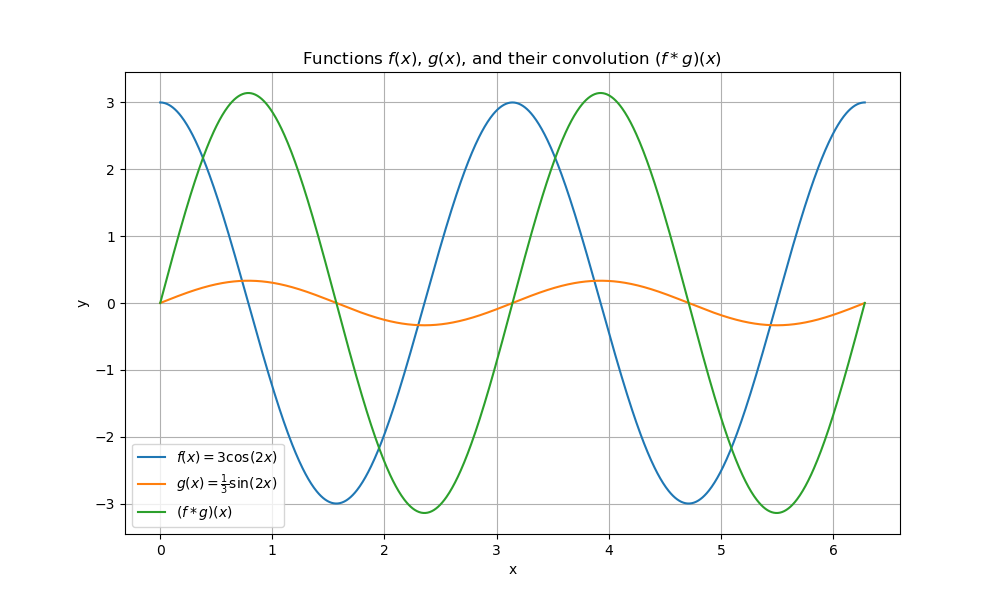
\includegraphics[width=1.0\linewidth]{Figure_3.png}
    \caption{Plot of y vs x}
    \label{fig:2}
\end{figure}\\
\end{document}
